\section{Domain Analysis}

\subsection{Objective of the Laboratory Work}

The objective of this laboratory work is to design, implement, and validate a signal conditioning pipeline for dual-sensor temperature monitoring on an Arduino Mega 2560 microcontroller. Building upon the sensor acquisition and threshold alerting foundations established in the previous laboratory, this work introduces a three-stage signal conditioning chain --- saturation clamping, median filtering, and exponentially weighted moving average (EWMA) smoothing --- that transforms raw sensor readings into clean, reliable temperature values suitable for threshold-based decision-making. The system reads temperature data from two distinct sensor types --- an analog NTC thermistor and a digital DS18B20 --- applies independent conditioning pipelines to each sensor channel, and presents all intermediate and final values through both an LCD display and structured STDIO reporting.

The key differentiator of this laboratory from the previous work is the explicit signal conditioning pipeline inserted between raw data acquisition and threshold alerting. Where the previous lab operated directly on converted temperature values, this lab demonstrates that raw sensor data in real-world embedded systems is inherently noisy and must be systematically conditioned before it can be trusted for decision-making. The three conditioning stages address different noise characteristics: saturation clamping rejects physically impossible outliers, median filtering removes impulsive salt-and-pepper noise spikes, and EWMA smoothing attenuates high-frequency random noise while preserving the underlying temperature trend.

The learning objectives include understanding the theoretical basis and practical implementation of each conditioning stage, analyzing the trade-offs between noise rejection and signal latency introduced by filtering, implementing modular signal conditioning libraries that can be independently configured per sensor channel, using FreeRTOS preemptive multitasking with mutex and semaphore synchronization to orchestrate the acquisition-conditioning-display pipeline, and formatting floating-point sensor data for display using the \texttt{dtostrf} function (since the AVR implementation of \texttt{printf} does not support the \texttt{\%f} format specifier).

\subsection{Problem Definition}

The task requires the development of a microcontroller-based temperature monitoring application with a configurable signal conditioning pipeline. The system must periodically acquire temperature data from two sensors: one analog sensor (NTC thermistor) read via the built-in 10-bit ADC, and one digital sensor (DS18B20) read via the OneWire protocol. The acquisition period must be configurable, with a default of 50 milliseconds to ensure adequate temporal resolution for the conditioning filters.

The acquired raw temperature data must pass through a three-stage conditioning pipeline before being used for threshold evaluation. The first stage is saturation clamping, which restricts the temperature value to a physically valid range (for example, $-40$\textdegree C to $+125$\textdegree C), rejecting any readings that fall outside this range by clamping them to the nearest boundary. The second stage is median filtering, which maintains a sliding window of the $N$ most recent saturated samples (default $N = 5$), sorts them, and outputs the middle value, thereby eliminating impulsive noise spikes that affect only one or two samples. The third stage is EWMA smoothing, which applies an exponentially weighted moving average with a configurable smoothing factor $\alpha$ (default $\alpha = 0.3$) to attenuate residual high-frequency noise while tracking the true temperature trend.

Each sensor channel must have its own independent conditioning pipeline instance, allowing different filter parameters to be configured per sensor if desired. Threshold alerting with hysteresis and software debounce must operate on the conditioned output values (after all three stages), not on the raw readings. This ensures that alert decisions are based on clean, filtered data rather than noisy raw samples.

The system must provide two output channels. An I2C LCD display shows the current conditioned temperature readings from both sensors and the alert status, alternating between information pages. Simultaneously, a structured report is printed to the serial terminal via STDIO at a configurable interval (every 2 seconds), providing detailed diagnostic information including raw values, saturated values, median-filtered values, EWMA-smoothed values, alert states, and cumulative statistics. All floating-point values in the STDIO output are formatted using \texttt{dtostrf} due to the AVR platform's lack of \texttt{\%f} support in \texttt{printf}.

The application architecture follows a modular design with clearly separated concerns, orchestrated by the FreeRTOS scheduler. The sensor acquisition task (highest priority) reads both sensors and stores the raw data. The conditioning task (medium priority) applies the three-stage pipeline and evaluates thresholds on the conditioned output. The display and reporting task (lowest priority) presents intermediate and final values to the user. Inter-task synchronization uses binary semaphores for event signaling and mutexes for shared data protection.

\subsection{Task Statement}

\begin{quote}
\textit{Sarcina de laborator --- Achiziție semnal analogic}

\textit{Pentru un senzor analogic sau digital de temperatură, să se realizeze o aplicație pentru MCU care va achiziționa periodic semnalul de la senzorul selectat dintr-o listă de senzori, va filtra semnalul și va afișa valorile intermediare și cea curentă prin STDIO fie către un afișor LCD, fie către o interfață serială.}

\textit{Varianta de realizare: implementarea unui sistem de monitorizare a doi senzori, unul analogic și unul digital, cu afișarea valorilor și alertelor de la ambii senzori pe display LCD.}
\end{quote}

The task statement requires the implementation of a periodic signal acquisition system for temperature sensors with signal filtering and display of intermediate values. The selected implementation variant extends this to a dual-sensor configuration combining an analog NTC thermistor and a digital DS18B20 sensor, with both sensor channels independently filtered through a three-stage conditioning pipeline. The system displays raw, intermediate, and final conditioned values through both an LCD display and a serial STDIO interface, providing full visibility into the conditioning process at every stage.

\subsection{Used Technologies}

\subsubsection{Signal Conditioning in Embedded Systems}

Raw sensor data in embedded systems is rarely suitable for direct use in decision-making. Analog sensors are subject to thermal noise, quantization error, electromagnetic interference, and component drift, while digital sensors can produce occasional erroneous readings due to communication glitches, timing violations, or internal conversion errors. Signal conditioning refers to the systematic chain of processing operations applied to raw sensor data to improve its quality, reliability, and suitability for downstream processing.

A well-designed conditioning pipeline typically includes multiple stages, each targeting a specific class of noise or artifact. The ordering of these stages matters: coarse rejection of impossible values should precede fine-grained filtering, and nonlinear filters (such as median) should precede linear smoothing filters (such as EWMA) to prevent outliers from corrupting the smoother's internal state. In this laboratory, the three-stage pipeline --- saturation, median filter, EWMA --- follows this principle and represents a practical, computationally efficient conditioning chain suitable for resource-constrained microcontrollers.

\subsubsection{Saturation (Signal Clamping)}

Saturation, also known as signal clamping, is the simplest and most fundamental conditioning operation. It restricts the input value to a predefined valid range by replacing any value below the minimum with the minimum and any value above the maximum with the maximum. In this laboratory, the saturation range is set to $[-40, +125]$\textdegree C, corresponding to the operational limits of the sensors used.

The purpose of saturation is twofold. First, it rejects physically impossible readings that may result from sensor faults, disconnected wiring, or ADC overflow conditions. For example, an open-circuit NTC thermistor produces an ADC reading of 1023, which the Steinhart-Hart equation maps to a temperature near $-273$\textdegree C --- a physically meaningless value that, if propagated through the pipeline, could corrupt downstream filter states. Second, saturation prevents the propagation of NaN (Not a Number) or infinity values that can arise from division-by-zero conditions in the temperature conversion equations. By clamping the output to a finite, bounded range, saturation ensures that all subsequent pipeline stages receive numerically well-behaved inputs. Despite its simplicity, saturation is an essential first line of defense in any signal conditioning chain.

\subsubsection{Median Filter (Salt-and-Pepper Noise Removal)}

The median filter is a nonlinear digital filter that is particularly effective at removing impulsive noise --- also known as salt-and-pepper noise --- from a signal. Unlike linear filters (such as the moving average), which spread the energy of a noise spike across multiple output samples, the median filter completely eliminates isolated outliers while preserving the underlying signal characteristics, including sharp edges and step changes.

The median filter operates by maintaining a sliding window of the $N$ most recent input samples. At each time step, the filter sorts the values within the window and outputs the middle element (the median). For a window size of $N = 5$, this means that up to 2 corrupted samples out of 5 can be present without affecting the output --- the median will still correspond to a valid measurement. This property makes the median filter ideal for rejecting sensor glitches that affect only a single sample or a small number of consecutive samples.

The choice of window size $N$ involves a trade-off between noise rejection capability and signal latency. A larger window tolerates more simultaneous outliers and provides better noise suppression, but introduces greater delay because the output reflects the median of a larger historical buffer. For temperature monitoring applications where the physical process changes slowly relative to the sampling rate, a window of $N = 5$ provides excellent impulse rejection with minimal latency (approximately $N/2 = 2.5$ sample periods of group delay). An odd window size is preferred because it guarantees a unique middle element, avoiding the need to average two central values as would be required with an even-sized window.

The computational cost of the median filter is dominated by the sorting step. For a window of size $N$, a comparison-based sort requires $O(N \log N)$ operations in the general case, though for the small window sizes typical in embedded applications ($N = 3$ to $N = 7$), simple insertion sort with $O(N^2)$ complexity is often preferred due to its low overhead and cache-friendly access pattern. The memory requirement is modest: only $N$ samples need to be stored in a circular buffer.

\subsubsection{Exponentially Weighted Moving Average (EWMA)}

The Exponentially Weighted Moving Average (EWMA) is a first-order infinite impulse response (IIR) low-pass filter that smooths a noisy signal by computing a weighted combination of the current input sample and the previous output. The EWMA is defined by the recursive formula:

$$y_n = \alpha \cdot x_n + (1 - \alpha) \cdot y_{n-1}$$

where $y_n$ is the filter output at time step $n$, $x_n$ is the current input sample, $y_{n-1}$ is the previous output, and $\alpha$ is the smoothing factor with $0 < \alpha \leq 1$. The parameter $\alpha$ controls the balance between responsiveness and smoothness: a larger $\alpha$ (closer to 1) makes the filter respond more quickly to input changes but provides less noise attenuation, while a smaller $\alpha$ (closer to 0) produces a smoother output but introduces greater lag in tracking genuine signal changes. In this laboratory, $\alpha = 0.3$ is used, providing a good compromise between noise rejection and response time for temperature monitoring.

The EWMA can be interpreted as a weighted sum of all past input samples, where the weight of each sample decreases exponentially with its age. The effective memory of the filter --- the number of past samples that contribute significantly to the output --- is approximately $2/\alpha$ samples. For $\alpha = 0.3$, this corresponds to roughly 6--7 samples, meaning the filter output reflects a weighted average of the most recent 6--7 readings.

Compared to a simple moving average (SMA) of equivalent smoothing, the EWMA offers two significant advantages for embedded systems. First, it requires only a single state variable (the previous output $y_{n-1}$) rather than a buffer of $N$ past samples, making it extremely memory-efficient. Second, its computational cost is constant --- just one multiplication and one addition per sample --- regardless of the effective averaging window. These properties make the EWMA an ideal smoothing filter for resource-constrained microcontrollers where both memory and CPU cycles are at a premium.

The EWMA is initialized with the first valid input sample ($y_0 = x_0$), which ensures that the filter output immediately reflects the actual signal level rather than ramping up from zero. After initialization, the filter converges to the steady-state signal level within approximately $3/\alpha$ samples.

\subsubsection{Analog-to-Digital Conversion (ADC)}

Analog-to-Digital Conversion is the process of translating a continuous analog voltage signal into a discrete digital representation that a microcontroller can process. The Arduino Mega 2560 features a 10-bit successive approximation ADC with 16 multiplexed input channels. The 10-bit resolution means the ADC maps the input voltage range (0 V to 5 V by default) into 1024 discrete levels, yielding a resolution of approximately 4.88 mV per step.

The ADC conversion process begins when the firmware triggers a conversion on the selected channel. The successive approximation register (SAR) algorithm performs a binary search through the possible output codes, comparing the input voltage against an internally generated reference at each step. On the ATmega2560, the ADC clock is derived from the system clock through a prescaler, and a full conversion requires 13 ADC clock cycles (25 cycles for the first conversion after enabling the ADC). At the default prescaler setting of 128 (yielding a 125 kHz ADC clock from the 16 MHz system clock), a single conversion takes approximately 104 microseconds.

For temperature measurement with an NTC thermistor, the ADC reading represents the voltage at the midpoint of a resistive voltage divider formed by the thermistor and a fixed series resistor. The raw ADC value is first converted to resistance using the voltage divider equation, and subsequently to temperature using the Steinhart-Hart Beta parameter equation:

$$\frac{1}{T} = \frac{1}{T_0} + \frac{1}{B} \cdot \ln\left(\frac{R_{NTC}}{R_0}\right)$$

where $T$ is the absolute temperature in Kelvin, $T_0$ is the reference temperature (typically 298.15 K = 25\textdegree C), $B$ is the Beta coefficient of the thermistor (3950 K for the sensor used in this lab), $R_{NTC}$ is the measured thermistor resistance, and $R_0$ is the nominal resistance at $T_0$ (10 k$\Omega$). The resistance is calculated from the ADC reading using:

$$R_{NTC} = R_{series} \cdot \frac{ADC}{ADC_{max} - ADC}$$

where $R_{series}$ is the fixed series resistor (10 k$\Omega$), $ADC$ is the raw digital reading, and $ADC_{max}$ is the maximum ADC value (1023 for 10-bit resolution). The resulting temperature in Kelvin is converted to Celsius by subtracting 273.15. On the AVR platform, the floating-point result is formatted for display using \texttt{dtostrf} rather than \texttt{printf} with \texttt{\%f}, as the AVR C library's \texttt{printf} implementation omits floating-point support to reduce code size.

\subsubsection{OneWire Communication Protocol}

OneWire is a proprietary communication protocol developed by Dallas Semiconductor (now Maxim Integrated / Analog Devices) that enables bidirectional data exchange between a master device and one or more slave devices over a single data wire plus ground. The protocol is particularly significant in embedded temperature sensing because it allows the DS18B20 digital temperature sensor to communicate its readings using only one GPIO pin, minimizing the wiring complexity of multi-sensor installations.

The OneWire protocol operates at TTL voltage levels and uses an open-drain bus topology with a pull-up resistor (typically 4.7 k$\Omega$) to VCC. Communication is initiated exclusively by the master, which drives the bus low to generate timing slots. The protocol defines several fundamental operations: Reset/Presence pulse (the master drives the bus low for at least 480 $\mu$s, then releases it; slave devices respond by pulling the bus low for 60--240 $\mu$s), Write Time Slot (the master drives the bus low and either releases it quickly for a logical `1' or holds it low for a logical `0'), and Read Time Slot (the master briefly drives the bus low, then samples the bus state; the slave holds the bus low for a `0' or releases it for a `1').

Each slave device on the OneWire bus has a unique 64-bit ROM code that serves as its address. For temperature measurement, the master issues a Convert T command (0x44), which instructs the DS18B20 to begin its internal analog-to-digital conversion. The conversion time depends on the configured resolution: 93.75 ms at 9-bit through 750 ms at 12-bit resolution. After conversion completes, the master reads the scratchpad memory containing the temperature result.

\subsubsection{I2C Communication Protocol}

Inter-Integrated Circuit (I2C) is a synchronous, multi-master, multi-slave serial communication protocol that uses two bidirectional open-drain lines: Serial Data (SDA) and Serial Clock (SCL). Developed by Philips Semiconductor (now NXP) in 1982, I2C has become one of the most widely used communication interfaces in embedded systems for connecting low-speed peripheral devices such as sensors, EEPROMs, real-time clocks, and LCD controllers.

\begin{figure}[H]
\centering
\IfFileExists{resources/DomainAnalysis/UsedTechnologies/i2c_protocol.png}{%
    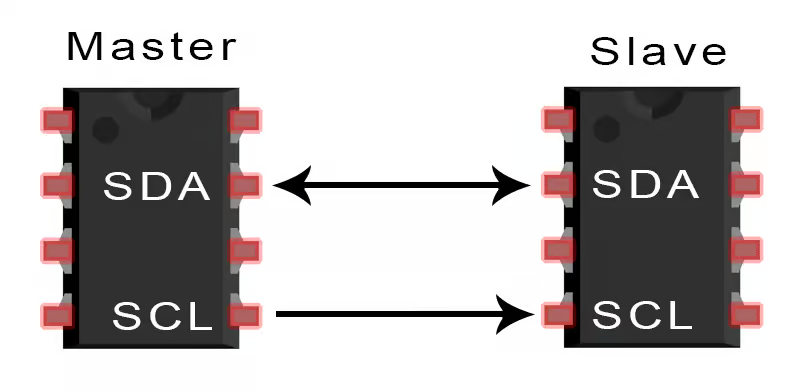
\includegraphics[width=0.7\textwidth]{resources/DomainAnalysis/UsedTechnologies/i2c_protocol.png}%
}{%
    \fbox{\parbox{0.68\textwidth}{\centering\color{gray}\small
        [Image pending --- save to resources/DomainAnalysis/UsedTechnologies/i2c\_protocol.png]}}%
}
\caption{I2C communication protocol timing diagram}
\label{fig:i2c_protocol}
\end{figure}

In this laboratory, I2C is used to communicate with the LCD 1602 display module through a PCF8574 I/O expander chip. The LCD module is configured at I2C address 0x27, and communication occurs at the standard 100 kHz clock speed. The Arduino Mega 2560 provides dedicated I2C pins: SDA on pin 20 and SCL on pin 21. Each I2C transaction follows a defined sequence: the master generates a START condition, transmits the 7-bit slave address followed by a read/write bit, waits for an acknowledgment from the addressed slave, transfers one or more data bytes, and generates a STOP condition. The LiquidCrystal\_I2C library abstracts these low-level protocol details, providing a simple API for text display operations, as shown in \citeimg{fig:i2c_protocol}.

\subsubsection{FreeRTOS Real-Time Operating System}

FreeRTOS is a real-time operating system (RTOS) kernel for embedded microcontrollers that provides preemptive multitasking, inter-task synchronization primitives, and deterministic scheduling. In this laboratory, FreeRTOS manages three concurrent tasks that together implement the sensor monitoring pipeline: acquisition, conditioning (including the three-stage filter chain and threshold evaluation), and display/reporting.

The FreeRTOS scheduler uses a priority-based preemptive algorithm: at any given moment, the highest-priority task that is ready to run receives CPU time. When a higher-priority task becomes ready (for example, when a semaphore it was waiting on is given), the scheduler immediately preempts the running lower-priority task and switches context to the higher-priority one. This mechanism ensures that time-critical operations such as sensor acquisition are never delayed by lower-priority work such as LCD display updates.

The synchronization primitives used in this lab include binary semaphores and mutexes. A binary semaphore acts as a lightweight signaling mechanism: the acquisition task \textit{gives} the semaphore after completing a reading cycle, and the conditioning task \textit{takes} the semaphore to wake up and process the new data. A mutex (mutual exclusion semaphore) protects the shared data structures accessed by multiple tasks, ensuring that only one task can read or modify the shared state at any time. FreeRTOS mutexes provide priority inheritance: if a low-priority task holds the mutex and a high-priority task attempts to acquire it, the low-priority task temporarily inherits the higher priority, preventing the pathological condition known as priority inversion.

\subsubsection{Hysteresis-Based Threshold Detection}

Hysteresis is a signal conditioning technique that uses two distinct thresholds --- an upper (high) threshold and a lower (low) threshold --- to determine state transitions, preventing rapid oscillation (chattering) when the signal hovers near a single threshold boundary. In the context of temperature monitoring, the alert state activates when the temperature rises above the high threshold (e.g., 30\textdegree C) and deactivates only when the temperature drops below the low threshold (e.g., 28\textdegree C).

A critical design decision in this laboratory is that hysteresis-based threshold detection operates on the \textit{conditioned} output values --- that is, the values that have already passed through the saturation, median filter, and EWMA stages --- rather than on the raw sensor readings. This ensures that threshold decisions are based on clean, filtered data, significantly reducing the risk of false alerts caused by transient noise spikes or sensor glitches. The debounce mechanism further strengthens robustness by requiring $N$ consecutive threshold crossings (configurable, default 5) before confirming a state transition, ensuring that even residual noise in the conditioned signal does not trigger spurious alerts.

\subsection{Hardware Components}

\subsubsection{Arduino Mega 2560}

The Arduino Mega 2560 is the central microcontroller development board used in this laboratory. It is based on the ATmega2560 AVR microcontroller, which features a 16 MHz clock frequency, 256 KB of Flash program memory, 8 KB of SRAM, and 4 KB of EEPROM. The board provides 54 digital I/O pins (15 of which support PWM output), 16 analog input pins with 10-bit ADC resolution, 4 hardware UART serial ports, an SPI interface, and an I2C interface.

For this laboratory, the Arduino Mega 2560 serves multiple roles: it reads the analog NTC thermistor through its ADC (pin A0), communicates with the DS18B20 via a digital GPIO pin (pin 2) using the OneWire protocol, drives an I2C LCD display through its dedicated SDA/SCL pins (pins 20/21), controls three indicator LEDs through digital GPIO pins (pins 8, 9, 10), and runs the FreeRTOS scheduler to manage the acquisition-conditioning-display task pipeline. The board's 8 KB SRAM is essential for running FreeRTOS with multiple tasks (each requiring its own stack allocation) and for maintaining the median filter buffers and EWMA state variables across both sensor channels.

\begin{figure}[H]
\centering
\IfFileExists{resources/DomainAnalysis/HardwareComponents/arduino_mega_2560.png}{%
    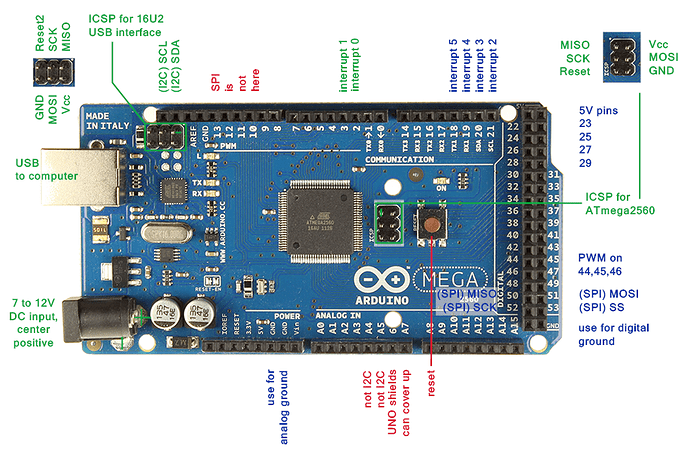
\includegraphics[width=0.65\textwidth]{resources/DomainAnalysis/HardwareComponents/arduino_mega_2560.png}%
}{%
    \fbox{\parbox{0.63\textwidth}{\centering\color{gray}\small
        [Photo pending --- save to resources/DomainAnalysis/HardwareComponents/arduino\_mega\_2560.png]}}%
}
\caption{Arduino Mega 2560 development board}
\label{fig:arduino_mega_2560}
\end{figure}

\subsubsection{NTC Thermistor (Analog Temperature Sensor)}

An NTC (Negative Temperature Coefficient) thermistor is a resistive temperature sensor whose electrical resistance decreases as temperature increases. The thermistor used in this laboratory has a nominal resistance of 10 k$\Omega$ at 25\textdegree C and a Beta coefficient ($B$ value) of 3950 K. These parameters define the resistance-temperature characteristic curve through the Steinhart-Hart Beta equation.

The NTC thermistor is connected in a voltage divider configuration with a 10 k$\Omega$ fixed series resistor. The midpoint voltage of this divider is fed to the Arduino's analog input pin A0. As the temperature changes, the thermistor resistance changes, altering the voltage division ratio and producing a corresponding change in the ADC reading. The analog nature of this sensor makes it particularly susceptible to electrical noise, quantization effects, and occasional erroneous readings caused by electromagnetic interference --- precisely the types of artifacts that the three-stage signal conditioning pipeline is designed to address.

\begin{figure}[H]
\centering
\IfFileExists{resources/DomainAnalysis/HardwareComponents/ntc_thermistor.png}{%
    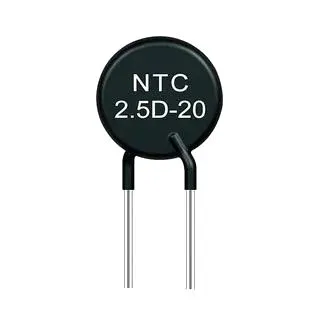
\includegraphics[width=0.4\textwidth]{resources/DomainAnalysis/HardwareComponents/ntc_thermistor.png}%
}{%
    \fbox{\parbox{0.38\textwidth}{\centering\color{gray}\small
        [Photo pending --- save to resources/DomainAnalysis/HardwareComponents/ntc\_thermistor.png]}}%
}
\caption{NTC thermistor (10K, Beta=3950)}
\label{fig:ntc_thermistor}
\end{figure}

\subsubsection{DS18B20 Digital Temperature Sensor}

The DS18B20 is a digital temperature sensor manufactured by Maxim Integrated that provides 9-to-12-bit temperature measurements over a single-wire digital interface. Unlike the NTC thermistor, which outputs an analog voltage that must be externally converted, the DS18B20 performs its own internal analog-to-digital conversion and communicates the result digitally, eliminating analog noise in the communication path. However, the DS18B20 can still produce occasional erroneous readings due to OneWire timing violations or CRC failures, making signal conditioning equally important for this digital sensor channel.

The DS18B20 measures temperatures from $-55$\textdegree C to $+125$\textdegree C with a configurable resolution. At 10-bit resolution (used in this lab), the sensor provides 0.25\textdegree C precision with a conversion time of approximately 187.5 ms. A 4.7 k$\Omega$ pull-up resistor on the DQ line is required because the OneWire bus uses an open-drain topology.

\begin{figure}[H]
\centering
\IfFileExists{resources/DomainAnalysis/HardwareComponents/ds18b20.png}{%
    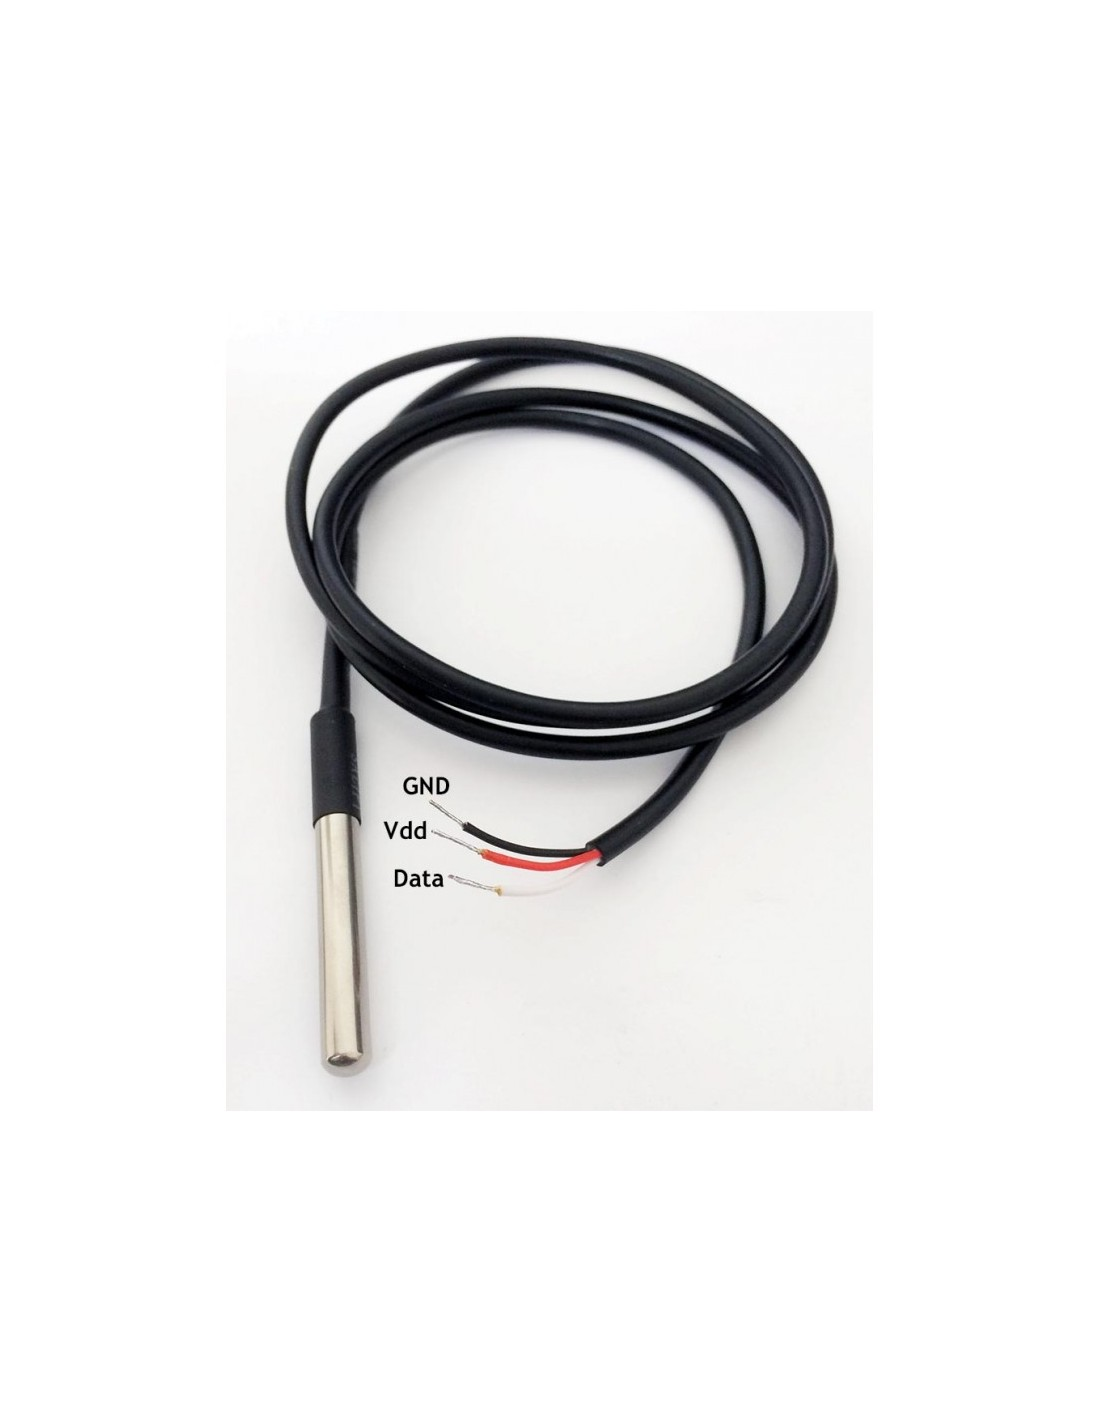
\includegraphics[width=0.4\textwidth]{resources/DomainAnalysis/HardwareComponents/ds18b20.png}%
}{%
    \fbox{\parbox{0.38\textwidth}{\centering\color{gray}\small
        [Photo pending --- save to resources/DomainAnalysis/HardwareComponents/ds18b20.png]}}%
}
\caption{DS18B20 digital temperature sensor (TO-92 package)}
\label{fig:ds18b20}
\end{figure}

\subsubsection{LCD 1602 with I2C Interface}

The LCD 1602 is a character liquid crystal display module capable of showing 16 characters per line across 2 lines. When equipped with a PCF8574-based I2C backpack module, the display communicates with the microcontroller over just two wires (SDA and SCL) instead of requiring 6--10 parallel data pins. The I2C address is typically 0x27.

In this laboratory, the LCD serves as the primary real-time display for conditioned temperature readings and alert status. The display alternates between information pages, showing current analog and digital temperatures (after the full conditioning pipeline) along with the overall system status. The 16-character line width constrains the information density, requiring careful formatting with \texttt{dtostrf} to present floating-point temperature values in a compact form.

\begin{figure}[H]
\centering
\IfFileExists{resources/DomainAnalysis/HardwareComponents/lcd_1602_i2c.png}{%
    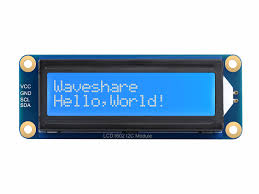
\includegraphics[width=0.5\textwidth]{resources/DomainAnalysis/HardwareComponents/lcd_1602_i2c.png}%
}{%
    \fbox{\parbox{0.48\textwidth}{\centering\color{gray}\small
        [Photo pending --- save to resources/DomainAnalysis/HardwareComponents/lcd\_1602\_i2c.png]}}%
}
\caption{LCD 1602 display with I2C backpack module}
\label{fig:lcd_1602_i2c}
\end{figure}

\subsubsection{LEDs with Current-Limiting Resistors}

Three LEDs provide immediate visual feedback on the system state. Each LED is connected to a digital GPIO pin through a 220~$\Omega$ current-limiting resistor, which restricts the forward current to approximately 15 mA at the 5 V logic level. The green LED (pin 8) indicates normal system operation with both sensors below their respective thresholds. The red LED (pin 9) indicates that the analog sensor has triggered a threshold alert based on its conditioned output. The yellow LED (pin 10) indicates that the digital sensor has triggered a threshold alert. During debounce transitions, the corresponding LED blinks to indicate that a state change is being validated but not yet confirmed.

\begin{figure}[H]
\centering
\IfFileExists{resources/DomainAnalysis/HardwareComponents/led.png}{%
    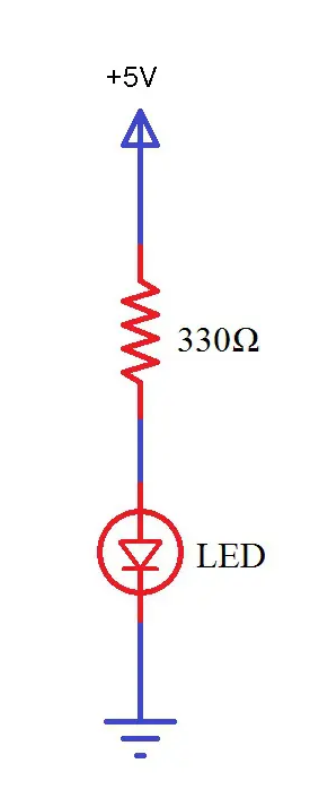
\includegraphics[width=0.35\textwidth]{resources/DomainAnalysis/HardwareComponents/led.png}%
}{%
    \fbox{\parbox{0.33\textwidth}{\centering\color{gray}\small
        [Photo pending --- save to resources/DomainAnalysis/HardwareComponents/led.png]}}%
}
\caption{Standard 5mm LEDs (green, red, yellow)}
\label{fig:led}
\end{figure}

\subsubsection{Resistors}

Several resistors are used in the circuit, each serving a distinct purpose. A 10 k$\Omega$ resistor forms the upper half of the voltage divider for the NTC thermistor, creating a known reference against which the thermistor's variable resistance produces a measurable voltage at the ADC input. A 4.7 k$\Omega$ pull-up resistor on the DS18B20 data line provides the required pull-up voltage for the open-drain OneWire bus, ensuring reliable signal levels during the precisely timed communication slots. Three 220 $\Omega$ resistors limit the current through the indicator LEDs to safe operating levels, protecting both the LEDs and the microcontroller GPIO pins from excessive current draw.

\subsection{Software Components}

\subsubsection{PlatformIO}

PlatformIO is a professional open-source ecosystem for embedded development that integrates with Visual Studio Code as an extension. It provides comprehensive project management, automatic library dependency resolution, multi-board and multi-environment support, and unified build/upload/monitor tools. In this laboratory, PlatformIO manages the compilation environment for the Arduino Mega 2560, automatically resolves library dependencies (FreeRTOS, OneWire, DallasTemperature, LiquidCrystal\_I2C), and provides the serial monitor for observing STDIO output. The PlatformIO project configuration (\texttt{platformio.ini}) defines a dedicated environment for Lab 3.2 with the required build flags and library dependencies, enabling the project to maintain multiple lab configurations simultaneously.

\begin{figure}[H]
\centering
\IfFileExists{resources/DomainAnalysis/SoftwareComponents/platformio.png}{%
    
\includegraphics[width=0.75\textwidth]{resources/DomainAnalysis/SoftwareComponents/platformio.png}%
}{%
    \fbox{\parbox{0.73\textwidth}{\centering\color{gray}\small
        [Screenshot pending --- save to resources/DomainAnalysis/SoftwareComponents/platformio.png]}}%
}
\caption{PlatformIO IDE in VS Code with Lab 3.2 project}
\label{fig:platformio}
\end{figure}

\subsubsection{Wokwi Simulator}

Wokwi is an embedded systems simulator available both as a web application and as a VS Code extension. It supports Arduino, ESP32, Raspberry Pi Pico, and other popular platforms, providing virtual components including LEDs, buttons, LCDs, temperature sensors (NTC thermistors and DS18B20), and serial terminals. Wokwi enables testing of the complete application --- including the signal conditioning pipeline --- in a simulated environment before deploying to physical hardware. The simulator's ability to inject controlled temperature changes and noise patterns is particularly valuable for validating the behavior of the saturation, median filter, and EWMA stages under various input conditions.

\begin{figure}[H]
\centering
\IfFileExists{resources/DomainAnalysis/SoftwareComponents/wokwi.png}{%
    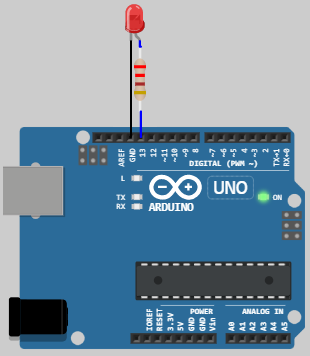
\includegraphics[width=0.75\textwidth]{resources/DomainAnalysis/SoftwareComponents/wokwi.png}%
}{%
    \fbox{\parbox{0.73\textwidth}{\centering\color{gray}\small
        [Screenshot pending --- save to resources/DomainAnalysis/SoftwareComponents/wokwi.png]}}%
}
\caption{Wokwi simulator running the Lab 3.2 circuit}
\label{fig:wokwi}
\end{figure}

\subsection{Case Study: Signal Conditioning in Industrial Process Control}

The three-stage signal conditioning pipeline implemented in this laboratory --- saturation clamping, median filtering, and EWMA smoothing --- directly mirrors techniques used in industrial process control systems where measurement reliability is paramount for safe and efficient operation.

In pharmaceutical manufacturing, regulatory frameworks such as FDA 21 CFR Part 211 mandate continuous environmental monitoring with documented evidence that temperature-sensitive products are stored within specified ranges. Pharmaceutical cold chain monitoring systems deploy arrays of temperature sensors across storage facilities, and raw sensor data must be conditioned before it is compared against regulatory thresholds. A single erroneous sensor reading that triggers a false out-of-specification alert can require discarding an entire batch of medication --- a potentially multi-million-dollar loss. Saturation clamping prevents sensor faults (such as a disconnected probe reading $-273$\textdegree C) from corrupting the monitoring record. Median filtering removes transient spikes caused by electromagnetic interference from nearby HVAC equipment or motor drives. EWMA smoothing tracks the true storage temperature while filtering out high-frequency noise, ensuring that threshold alerts reflect genuine temperature excursions rather than measurement artifacts.

Food safety monitoring presents similar challenges. HACCP (Hazard Analysis and Critical Control Points) regulations require that critical control points --- such as cooking temperatures, refrigeration units, and blast chillers --- be continuously monitored with documented alarm response procedures. In a commercial food processing facility, temperature sensors are exposed to steam, vibration, and electrical noise from high-power cooking equipment. The conditioning pipeline ensures that the monitoring system alerts operators to genuine temperature violations while suppressing the nuisance alarms that can lead to alarm fatigue and, paradoxically, reduced safety compliance.

HVAC (Heating, Ventilation, and Air Conditioning) building management systems represent yet another application domain. Modern building automation controllers read hundreds of temperature, humidity, and pressure sensors distributed throughout a facility. The raw sensor data is conditioned through configurable filter chains before being fed to PID control loops and alarm engines. An unconditioned noisy temperature signal driving a PID controller would cause the HVAC actuators (dampers, valves, compressors) to oscillate rapidly, increasing mechanical wear, energy consumption, and occupant discomfort. The EWMA filter's ability to smooth high-frequency noise while tracking slow temperature trends makes it a standard component in commercial building controllers, and its minimal computational and memory requirements (a single state variable per channel) allow it to be deployed across hundreds of sensor channels simultaneously on resource-constrained embedded platforms.
